\subsubsection{Zellen}
\label{sec:zellen}

Zellen sind dynamische Spielobjekte, die entweder vom Spieler oder von der KI
kontrolliert werden oder sich neutral verhalten. Sie haben eine oder mehr
der Eigenschaften aus \tabref{tab:eigenschaften}.

Die Eigenschaften unterteilen sich in persistente, die sich während des
Lebenszyklus einer Zelle nicht ändern, und nicht persistente, die sich
nach der Entstehung einer Zelle noch ändern können. Alle persistenten
Eigenschaften können sich aber bei der Zellteilung oder der Produktion von Viren
durch Mutation ändern.

\begin{table}
  \begin{tabu} to \linewidth {|l|X|}
    \hline
    Eigenschaft &
      Beschreibung\\\hline

    Maximale Lebenspunkte &
      Maximale Lebenspunkte einer Zelle. Wertebereich 1 (schwach) bis 100
      (stark).\\\hline

    Aktuelle Lebenspunkte &
      Lebenspunkte einer Zelle von 0 (tot) bis zum durch die Eigenschaft
      Maximale Lebenspunkte vorgegebenen Maximalwert. Direkt nach ihrer
      Entstehung entsprechen die aktuellen Lebenspunkte einer Zelle ihren
      maximalen Lebenspunkten. Durch Angriffe gegnerischer Zellen können
      die aktuellen Lebenspunkte reduziert werden. Erreichen die aktuellen
      Lebenspunkte den Wert 0, stirbt die Zelle. Diese Eigenschaft ist
      nicht persistent.\\\hline

    Initiale Lebensdauer &
      Zeitspanne, nach der eine Zelle unabhängig von ihren aktuellen
      Lebenspunkten \enquote*{natürlich} stirbt, in Sekunden ab ihrer
      Entstehung.\\\hline

    Verbleibende Lebensdauer &
      Zeitspanne, nach der eine Zelle unabhängig von ihren aktuellen
      Lebenspunkten \enquote*{natürlich} stirbt, in Sekunden ab dem aktuellen
      Zeitpunkt. Verringert sich jede Sekunde um eins. Bei Entstehung der
      Zelle entspricht dieser Wert der Initialen Lebensdauer. Diese
      Eigenschaft ist nicht persistent.\\\hline

    Angriffsstärke &
      Anzahl der Lebenspunkte pro Sekunde, die die Zelle einer gegnerischen
      Zelle beim Angriff abzieht.\\\hline

    Geschwindigkeit &
      Bewegungsgeschwindigkeit einer Zelle. Wertebereich 1 (langsam) bis 100
      (schnell).\\\hline

    Zellteilungsgeschwindigkeit &
      Dauer einer Zellteilung in Sekunden, von ihrer Initiation bis zum
      Entstehen der neuen Zelle.\\\hline

    Sichtweite &
      Sichtweite einer Zelle. Wertebereich 1 (kurz) bis (100 lang).\\\hline

    Antigen &
      Spezielle Eigenschaft von Viren, Bakterien, B-, T-, und Riesenfresszellen
      sowie Antikörpern. Siehe \secref{sec:spielmechaniken} und
      \secref{sec:optionen_aktionen} für Details zu den assoziierten
      Spielmechaniken.\\\hline

    Virenresistenz &
      Resistenz einer Zelle gegen Virenangriffe. Übersteigt die
      Infektionsstärke eines angreifenden Virus die Virenresistenz der
      angegriffenen Zelle, so wird die Zelle vom Virus übernommen. Wertebereich
      1 (schwach) bis 100 (stark).\\\hline

    Infektionsstärke &
      Angriffsstärke eines Virus. Übersteigt dieser Wert die Virenresistenz
      einer gegnerischen Zelle, so kann die Zelle vom Virus übernommen werden.
      Wertebereich 1 (schwach) bis 100 (stark).\\\hline

  \end{tabu}
  \caption{Eigenschaften. Wo nicht anders gekennzeichnet, sind die
  Eigenschaften persistent.}
  \label{tab:eigenschaften}
\end{table}

Im Folgenden werden alle Zellen des Spiels aufgeführt. Die angegebenen
Eigenschaftswerte für Lebensdauer und Zellteilungsgeschwindigkeit geben nur
näherungsweise die Verhältnisse zwischen verschiedenen Einheiten an, nicht aber
die absoluten Werte in Sekunden.

% Params:
%    1 Name
%    2 Dateiname des Bildes
%    3 kontrolliert durch
%    4 Beschreibung
%    5 Max. Lebenspunkte
%    6 Initiale Lebensdauer
%    7 Angriffsstärke
%    8 Geschwindigkeit
%    9 Zellteilungsgeschwindigkeit
%   10 Sichtweite
%   11 Virenresistenz
%   12 Infektionsstärke
%   13 attackiert
%   14 attackiert von
%   15 produziert von
%   16 produziert
\newcommand\cellentry[9]{%
  \minisec{#1}%
  #4%

  %\multicolumn{2}{|c|}{#1}\\%
  %\multicolumn{2}{|c|}{\includegraphics[width=2cm]{img_objekte/#2}}\\%
  \begin{tabular} {|l|p{9cm}|}%
    \hline%
    kontrolliert durch          & #3\\\hline%
    Maximale Lebenspunkte       & #5\\\hline%
    Initiale Lebensdauer        & #6\\\hline%
    Angriffsstärke              & #7\\\hline%
    Geschwindigkeit             & #8\\\hline%
    Zellteilungsgeschwindigkeit & #9\\\hline%
}%

\newcommand\cellentryctd[7]{%
    Sichtweite                  & #1\\\hline%
    Virenresistenz              & #2\\\hline%
    Infektionsstärke            & #3\\\hline%
    attackiert                  & #4\\\hline%
    attackiert von              & #5\\\hline%
    produziert von              & #6\\\hline%
    produziert                  & #7\\\hline%
  \end{tabular}%
}

\cellentry
  {Stammzelle}
  {stemcellorig}
  {Spieler}
  {Produziert durch Zellteilung alle vom Spieler kontrollierten
   Zellen (außer Antikörpern) sowie rote Blutkörperchen.
   Die Zellteilung einer Stammzelle dauert
   wesentlich kürzer als die anderer Einheiten. Stammzellen können nicht
   angreifen.
  }
  {70} % Max. Lebenspunkte
  {70} % Initiale Lebensdauer
  {--} % Angriffsstärke
  {20} % Geschwindigkeit
  {70} % Zellteilungsgeschwindigkeit
\cellentryctd
  {50} % Sichtweite
  {60} % Virenresistenz
  {--} % Infektionsstärke
  {--} % attackiert
  {Bakterium, Virus} % attackiert von
  {Stammzelle} % produziert von
  {Stamm-, B-, T-, Riesenfresszelle; rote Blutkörperchen} % produziert

\cellentry
  {B-Zelle}
  {bcellorig}
  {Spieler}
  {B-Zellen können Antikörper produzieren, sofern sie ein Antigen besitzen. Das
   Antigen kann von einer Riesenfresszelle, die zuvor eine gegnerische Zelle
   getötet hat, übernommen werden. Es wird an die produzierten Antikörper
   sowie an durch Zellteilung produzierte B-Zellen weitergegeben. B-Zellen
   können nicht angreifen.
  }
  {30} % Max. Lebenspunkte
  {30} % Initiale Lebensdauer
  {--} % Angriffsstärke
  {40} % Geschwindigkeit
  {20} % Zellteilungsgeschwindigkeit
\cellentryctd
  {50} % Sichtweite
  {30} % Virenresistenz
  {--} % Infektionsstärke
  {--} % attackiert
  {Bakterium, Virus} % attackiert von
  {Stammzelle, B-Zelle} % produziert von
  {Antikörper, B-Zelle} % produziert

\cellentry
  {T-Zelle}
  {tcellorig}
  {Spieler}
  {Spezialisierte Angriffseinheit gegen infizierte Zellen. Kann ausschließlich
   infizierte Zellen, deren Antigen sie besitzt, attackieren. Erhält ihr Antigen
   von einer Riesenfresszelle, nachdem diese eine gegnerische Zelle getötet
   und ihr Antigen extrahiert haben. Gibt bei der Zellteilung ihr Antigen
   an die neu entstandene Zelle ab.
  }
  {60} % Max. Lebenspunkte
  {40} % Initiale Lebensdauer
  {30 (+ 30 mit Antigenbonus)} % Angriffsstärke
  {50} % Geschwindigkeit
  {20} % Zellteilungsgeschwindigkeit
\cellentryctd
  {50} % Sichtweite
  {50} % Virenresistenz
  {--} % Infektionsstärke
  {Infizierte Zelle} % attackiert
  {Bakterium, Virus} % attackiert von
  {Stammzelle, T-Zelle} % produziert von
  {T-Zelle} % produziert

\cellentry
  {Riesenfresszelle}
  {fresszelleorig}
  {Spieler}
  {Angriffseinheit, die Bakterien und Viren, aber keine infizierten Zellen
   attackieren kann. Kann keine Zellteilung durchführen. Tötet eine
   Riesenfresszelle eine gegnerische Einheit, so nimmt sie deren Antigen
   auf und kann dieses an eine T- oder B-Zelle weitergeben.
  }
  {50} % Max. Lebenspunkte
  {30} % Initiale Lebensdauer
  {40} % Angriffsstärke
  {50} % Geschwindigkeit
  {--} % Zellteilungsgeschwindigkeit
\cellentryctd
  {50} % Sichtweite
  {30} % Virenresistenz
  {--} % Infektionsstärke
  {Bakterium, Virus} % attackiert
  {Bakterium, Virus} % attackiert von
  {Stammzelle} % produziert von
  {--} % produziert

\cellentry
  {Antikörper}
  {antikoerperorig}
  {Spieler}
  {Angriffseinheit, die gegnerische Zellen befallen kann. Durch den Befall
   werden die Werte der persistenten Eigenschaften der befallenen Zelle
   dauerhaft verringert (\enquote*{Debuff}) und der befallende Antikörper
   vernichtet. Antikörper übernehmen das Antigen der sie produzierenden B-Zelle
   und können nur Zellen mit diesem Antigen angreifen. Antikörper können keine
   Zellteilung durchführen.
  }
  {30} % Max. Lebenspunkte
  {40} % Initiale Lebensdauer
  {--} % Angriffsstärke
  {70} % Geschwindigkeit
  {--} % Zellteilungsgeschwindigkeit
\cellentryctd
  {50} % Sichtweite
  {20} % Virenresistenz
  {--} % Infektionsstärke
  {Bakterium/Virus mit dem Antigen des Antikörpers} % attackiert
  {Bakterium, Virus} % attackiert von
  {B-Zelle mit Antigen} % produziert von
  {--} % produziert

\cellentry
  {Rotes Blutkörperchen}
  {redbloodcella}
  {neutral}
  {Neutrale Zelle, die vom Spieler produziert und von Bakterien und Viren
   angegriffen werden kann. Wird nicht vom Spieler kontrolliert und bewegt
   sich passiv mit dem Blutstrom. Kann keine Zellteilung durchführen und
   gewährt dem Spieler keine Sicht in seinem Umkreis.
  }
  {30} % Max. Lebenspunkte
  {40} % Initiale Lebensdauer
  {--} % Angriffsstärke
  {50} % Geschwindigkeit
  {--} % Zellteilungsgeschwindigkeit
\cellentryctd
  {--} % Sichtweite
  {20} % Virenresistenz
  {--} % Infektionsstärke
  {--} % attackiert
  {Bakterium, Virus} % attackiert von
  {Stammzelle} % produziert von
  {--} % produziert

\cellentry
  {Bakterium}
  {bakteriumorig}
  {KI}
  {Angriffseinheit der gegnerischen KI. Besitzt die Eigenschaft Antigen, die
   bei der Zellteilung im Regelfall an das produzierte Bakterium vererbt
   wird. Es besteht allerdings eine geringe Wahrscheinlichkeit, dass das
   produzierte Bakterium zufällig ein anderes Antigen als das produzierende
   erhält.
  }
  {50} % Max. Lebenspunkte
  {30} % Initiale Lebensdauer
  {40} % Angriffsstärke
  {50} % Geschwindigkeit
  {30} % Zellteilungsgeschwindigkeit
\cellentryctd
  {50} % Sichtweite
  {--} % Virenresistenz
  {--} % Infektionsstärke
  {Stammzelle, Riesenfresszelle, T-Zelle, B-Zelle, Antikörper, rotes Blutkörperchen} % attackiert
  {Riesenfresszelle, Antikörper} % attackiert von
  {Bakterium} % produziert von
  {Bakterium} % produziert

\cellentry
  {Virus}
  {virusaorig}
  {KI}
  {Angriffseinheit der KI. Kann die Lebenspunkte gegnerischer Zellen nicht
   reduzieren, aber sie infizieren. Wird eine Einheit infiziert, so
   transformiert sie sich in eine infizierte Zelle, die nicht mehr vom
   Spieler kontrolliert wird. Das infizierende Virus wird dabei vernichtet.
   Jedes Virus besitzt ein Antigen, das bei
   der Infektion einer Zelle an die dadurch entstehende infizierte Zelle
   weitergegeben wird. Viren können keine Zellteilung durchführen. Die
   Eigenschaft \emph{Zellteilungsgeschwindigkeit} ist stattdessen dafür
   maßgeblich, wie schnell eine durch ein Virus infizierte Zelle neue
   Viren produziert.
  }
  {40} % Max. Lebenspunkte
  {40} % Initiale Lebensdauer
  {--} % Angriffsstärke
  {40} % Geschwindigkeit
  {40} % Zellteilungsgeschwindigkeit
\cellentryctd
  {50} % Sichtweite
  {--} % Virenresistenz
  {30} % Infektionsstärke
  {Stammzelle, Riesenfresszelle, T-Zelle, B-Zelle, Antikörper, rotes Blutkörperchen} % attackiert
  {Riesenfresszelle, Antikörper} % attackiert von
  {infizierte Zelle} % produziert von
  {infizierte Zelle (durch Infektion)} % produziert

\cellentry
  {Infizierte Zelle}
  {infectedcell}
  {KI}
  {Produktionseinheit der KI. Entsteht durch Infektion einer Zelle des
   Spielers oder eines roten Blutkörperchens. Erbt die Antigeneigenschaft
   von dem infizierenden Virus und alle anderen Eigenschaften von der
   Zelle, die von dem Virus infiziert wurde. Produziert kontinuierlich Viren,
   auf die das Antigen der infizierten Zelle im Regelfall vererbt wird. Mit
   geringer Wahrscheinlichkeit werden allerdings auch Viren mit einem
   zufälligen anderen Antigen produziert. Infizierte Zellen können nicht
   angreifen.
  }
  {geerbt bei Infektion} % Max. Lebenspunkte
  {geerbt bei Infektion} % Initiale Lebensdauer
  {--} % Angriffsstärke
  {geerbt bei Infektion} % Geschwindigkeit
  {geerbt von infizierendem Virus} % Zellteilungsgeschwindigkeit
\cellentryctd
  {geerbt bei Infektion}
  {--} % Virenresistenz
  {--} % Infektionsstärke
  {--} % attackiert
  {T-Zelle} % attackiert von
  {Virus (durch Infektion)} % produziert von
  {Virus} % produziert

\subsubsection{Sonstige Objekte}

\minisec{Blutbahn}

\begin{figure}
  \begin{center}
  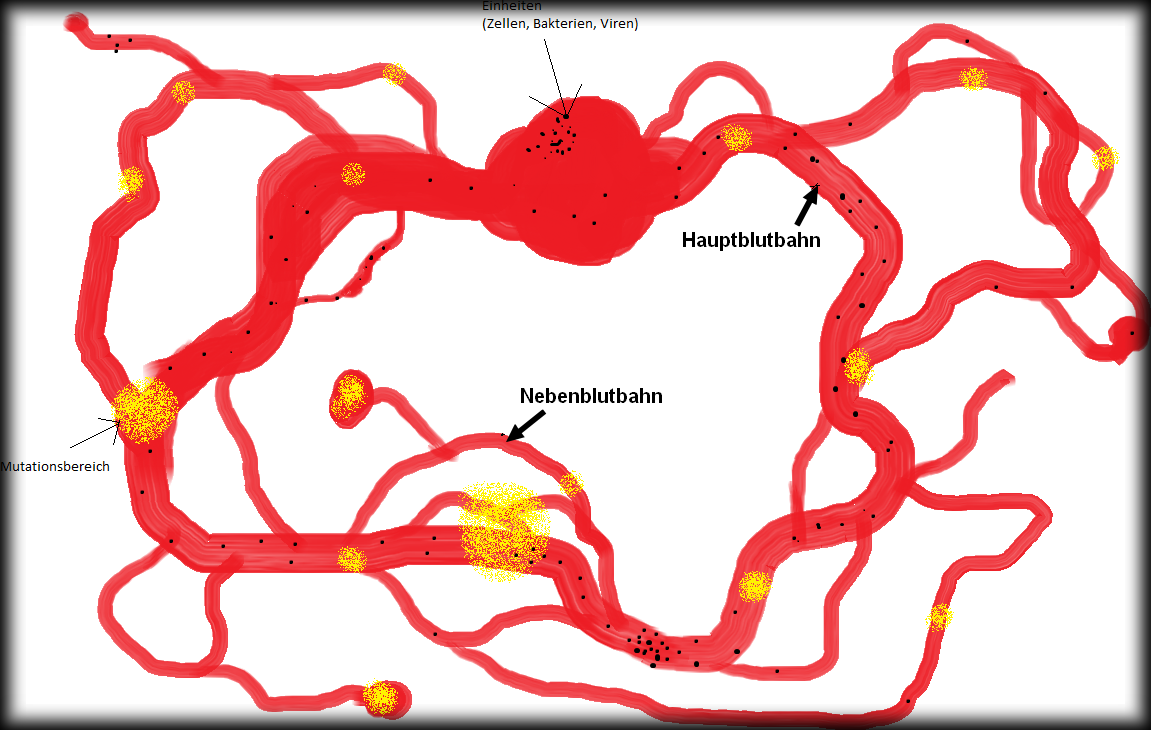
\includegraphics[width=10cm]{./img_objekte/blutbahn.png}\\
  \end{center}

  \caption{Blutbahnen}
  \label{fig:blutbahnen}
\end{figure}

Blutbahnen (Illustration s. \figref{fig:blutbahnen}) sind die begehbaren
Bereiche der Spielkarte. In Blutbahnen herrscht ein gerichteter Blutfluss, mit
dem sich Zellen treiben lassen können. (Siehe \secref{sec:aktionen}.)

\minisec{Mutationsfeld}

\begin{figure}
  \begin{center}
    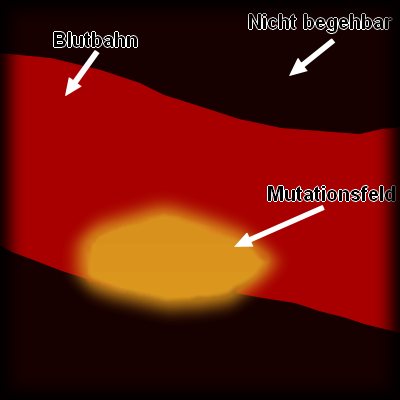
\includegraphics[width=5cm]{./img_objekte/mutationsfeld.png}\\
  \end{center}

  \caption{Mutationsfeld}
  \label{fig:mutationsfeld}
\end{figure}

Mutationsfelder (Illustration s. \figref{fig:mutationsfeld}) sind zufällig
auf Blutbahnen verteilte, persistente, begehbare Bereiche. Teilt sich eine Zelle,
während sie auf einem solchen Feld steht, so mutiert sie mit hoher
Wahrscheinlichkeit.

Verschiedene Mutationsfelder priorisieren verschiedene Eigenschaften
(beispielsweise Angriffsstärke), die wahrscheinlicher als andere Eigenschaften
bei der Mutation geändert werden. Jedes Mutationsfeld bietet jedoch eine
deutlich erhöhte Wahrscheinlichkeit der Änderung des Antigens von Viren
und Bakterien.
